\chapter{Tehnologii utilizate}

\section{Flutter}

\textbf{Flutter} este o platformă pentru dezvoltare de aplicații publicată inițial în 2017. Cu ajutorul acestui \textbf{SDK} (\emph{Software Development Kit}), programatorii pot construi aplicații web, desktop și cross-platform pentru Android și IOS. Se folosește împreună cu limbajul de programare Dart.

Pentru a dobândi o eficiență asemănătoare celei native, este folosită compilarea \textbf{AOT} (\emph{ahead-of-time}) pe toate platformele în afară de Web, unde codul este convertit în JavaScript.

Fundația acestui SDK este scrisă în \textbf{C++}, oferă randare low-level folosind biblioteca \emph{Skia} de la Google sau un strat de abstractizare grafic \emph{Impeller}. Componenta de bază în Flutter este \emph{widget-ul} care poate conține și alte widget-uri. Acesta descrie logica, interacțiunea și design-ul unei componente UI. Flutter conține două pachete de elemente UI: Material Design (Google) și Cupertino (Apple).

\begin{lstlisting}[language=C++, caption=Widget Scaffold]
	return Scaffold(
		body: Column(
		children: [
			Text('Acest text va fi pozitionat'),
			Text('Deasupra acestui text'),
			],
		),
	);
\end{lstlisting}

\section{Flask}

Flask este un framework web ușor de utilizat și flexibil, scris în Python. A fost creat cu scopul de a fi simplu și minimalist, oferind totodată funcționalitățile esențiale necesare pentru dezvoltarea rapidă a aplicațiilor. Acesta permite definirea de rute pentru a mapa cererile HTTP/HTTPS primite către funcții. Prin intermediul adnotărilor, se pot atribui funcțiilor URL-uri și metode HTTP/S specifice, permițând astfel aplicației să proceseze cererea în funcție de parametrii primiți.

Datorită abordării sale minimaliste și comunității active, Flask a devenit unul dintre cele mai populare framework-uri pentru dezvoltarea aplicațiilor web în Python.

Figura 2.2 reprezintă un script ce expune o rută care returnează un paragraf HTML cu textul \emph{Hello, World!}.

\begin{lstlisting}[language=Python, caption=Exemplu minimal de aplicație Flask]
	from flask import Flask	
	app = Flask(name)
	@app.route("/")
	def hello_world():
		return "<p>Hello, World!</p>"
\end{lstlisting}
\section{Raspberry Pi Zero W}

Raspberry Pi este o familie de calculatoare, de mărimea unui card de credit sau mai mici, care au revoluționat industria cu prețul accesibil de doar \$25 al primei plăci. În ultimii 5 ani, acestea au dobândit o atenție foarte mare în rândul comunității \emph{Do it yourself (DIY)} datorită spectrului larg de utilizări în proiecte digitale și IoT.

Comunitatea Raspberry a crescut mult și consistent. În momentul de față, în urma căutării "Raspberry pi projects", ne sunt returnate 47.2 milioane de pagini care conțin tutoriale despre imprimante 3D, sisteme de irigare, de luat vederi, ad-blocker pentru rețea și multe altele.

În contextul versiunii Zero W (Figura 2.1), avem disponibilă o placă de mărimea unui pachet de gume: 6.5 x 3 x 0.5 cm pe care poate fi instalat un sistem de operare bazat pe GNU/Linux numit Raspbian OS. Are un procesor single-core de 1GHz, 512 MB LPDDR2 RAM, iesire mini HDMI, două porturi micro USB, Bluetooth 4.0 și 2.4GHz 802.11n Wi-Fi.

Aspectul special al acestor computere constă în cei 40 pini \textbf{GPIO} (\emph{General purpose input-output}). Aceștia sunt folosiți pentru conectarea de senzori, fiind ușor programabili cu ajutorul limbajului Python, sau pentru audiențe tinere, Scratch.


\begin{figure}[h]
	\centering
	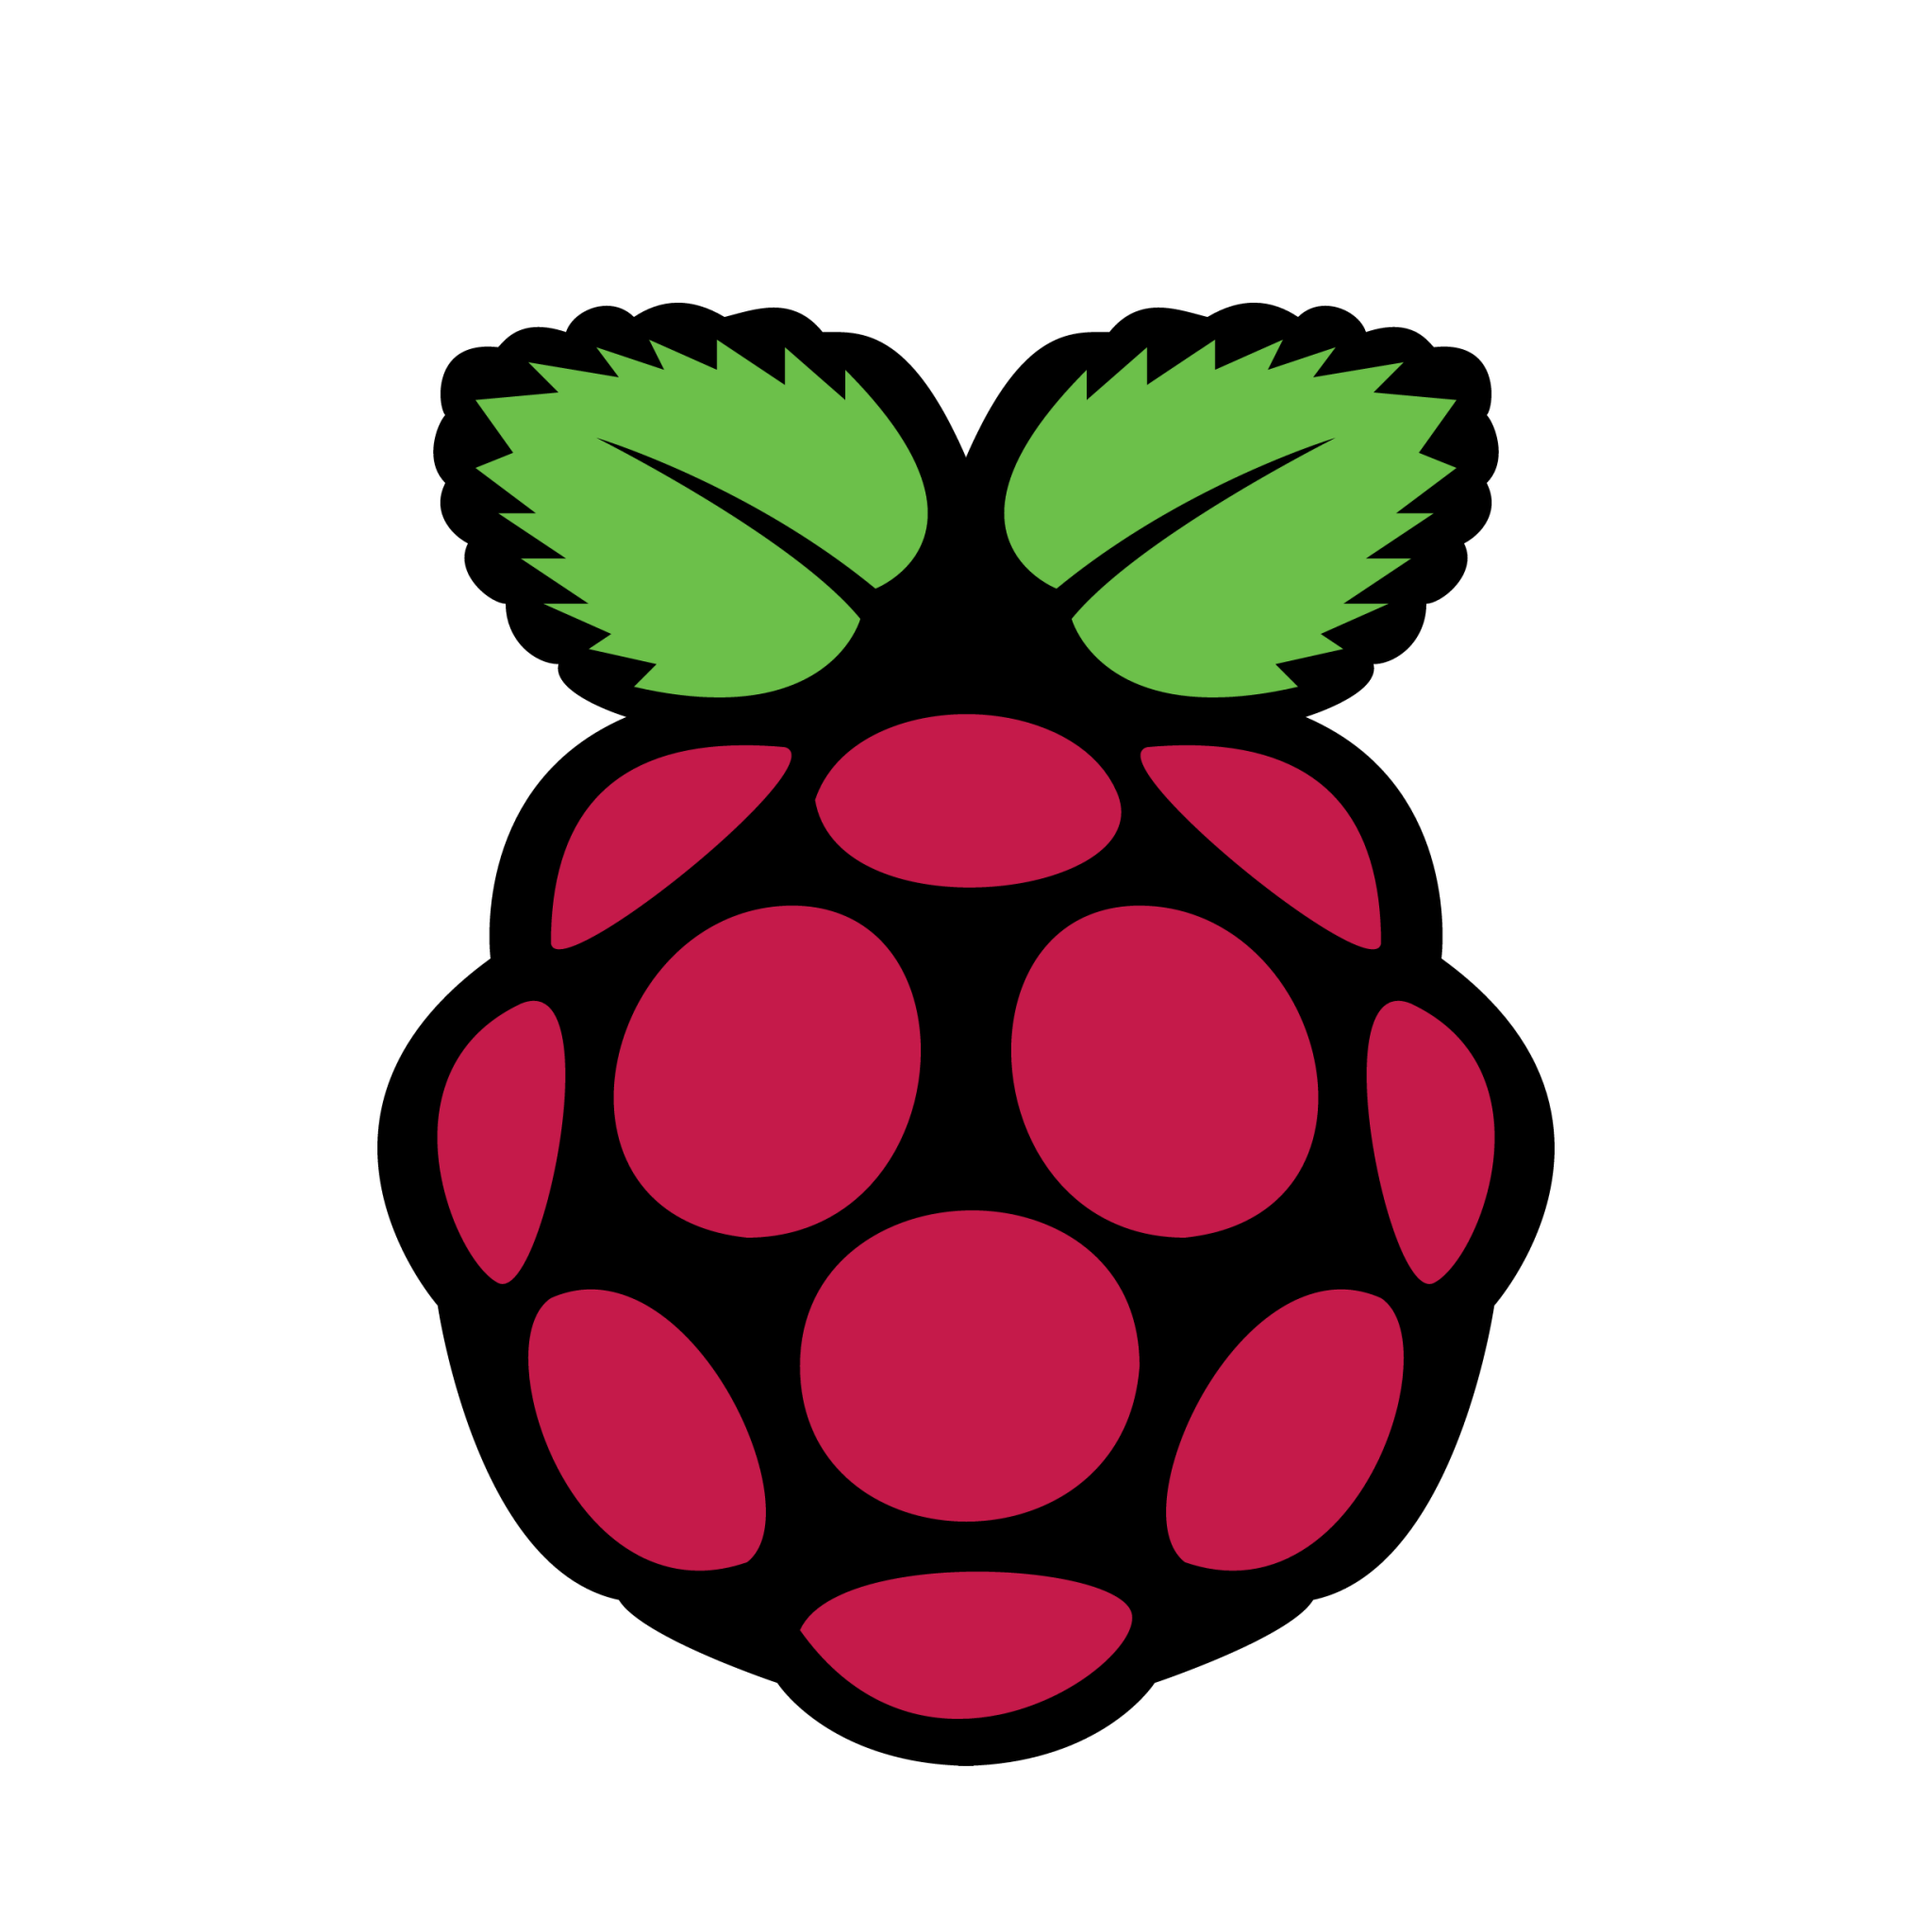
\includegraphics[width=1\textwidth]{raspberrypi}
	\caption{Fața și spatele plăcii Raspberri Pi Zero W
		Credits: RPISpy @ \url{https://www.raspberrypi-spy.co.uk/}}
	\label{fig:raspberrypi}
\end{figure}

\break

\section{Microcontrollere folosite}

Un microcontroller (abreviat \emph{MCU}) este un circuit integrat care combină funcționalitate microporcesorului (de obicei aflat sub un radiator de aluminiu pentru disiparea căldurii) cu componentele periferice: module \emph{Input/output}, memorie și interfețe de comunicare cu alte module. Dețin mai mulți pini de tip analog, digital și \textbf{PWM} (\emph{Pulse Width Modulation}) pentru conectarea cu alte module

\subsection{Arduino Nano}

Arduino Nano (Figura 2.2) este fratele mai mic al plăcii Uno cu care împărtășește majoritatea funcționalității: microcontroller ATmega328, 32KB memorie flash, viteză de 16MHz și 22 pini I/O.  Singurele diferențe sunt mărimea redusă și portul de USB mini. Este perfect pentru persoanele care doersc să învețe tainele electronicii și a programării, fiind potrivit pentru proiecte ce au constrângeri legate de spațiul disponibil.

\begin{figure}[h]
	\centering
	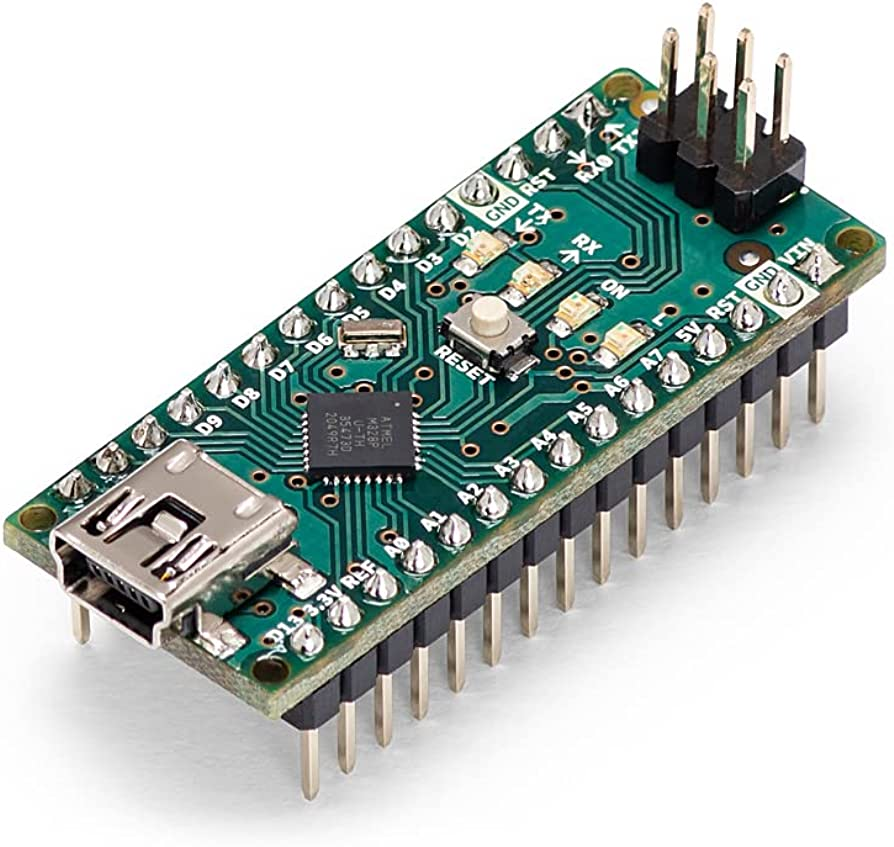
\includegraphics[width=0.4\textwidth]{arduino}
	\caption{Arduino Nano \newline\url{https://www.amazon.com/Arduino-A000005-ARDUINO-Nano/dp/B0097AU5OU}}
	\label{fig:arduino}
\end{figure}

\subsection{ESP8266}

Modulul ESP8266 (Figura 2.3) este un \textbf{SOC} (\emph{System on a chip}) produs de firma Espressif Systems ce folosește stack-ul TCP/IP cu ajutorul căruia se poate conecta la internet.

Acesta a fost popularizat în anul 2014 de către alt SOC asemănător \textbf{ESP-01} al firmei \textbf{Ai-Thinker}. Chip-urile se pot conecta la rețele Wifi și să realizeze conexiuni prin utilizarea comenzilor de tipul \emph{Hayes}, \textbf{AT commands}.

La început, nu existau documentații în limba engleză. Dat fiind faptul că SoC-ul este ieftin și deține un număr mic de componente externe, acesta poate fi produs în volume mari la preț mic, ceea ce a atras mulți hackeri să-l exploreze și să traducă documentația. 

\begin{figure}[h]
	\centering
	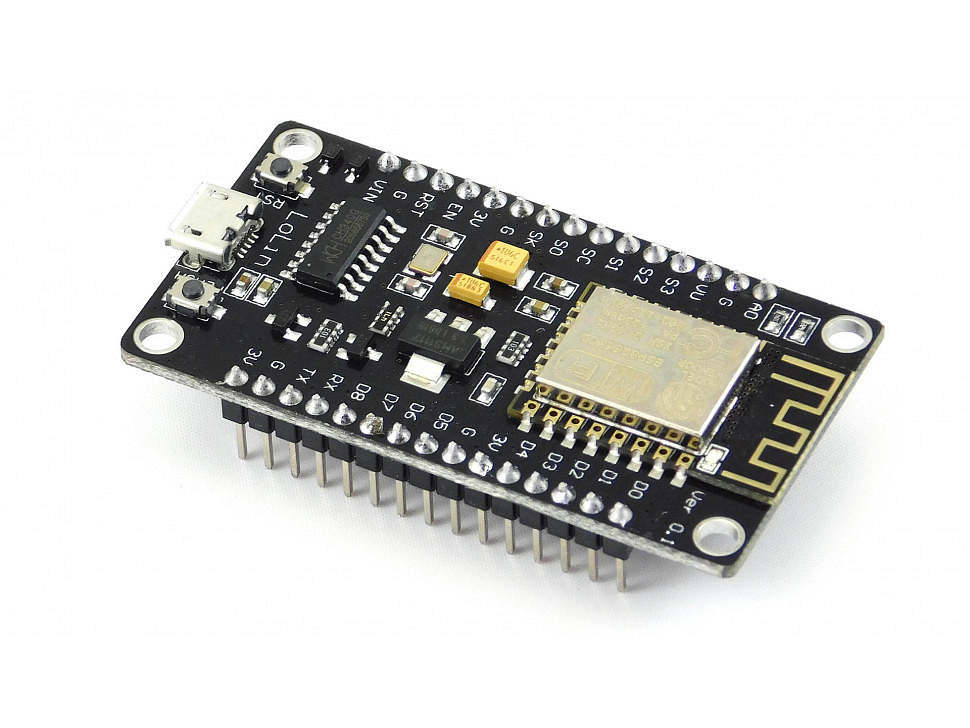
\includegraphics[width=1\textwidth]{esp8266}
	\caption{Microcontroller-ul ESP8266 (chip-ul argintiu) pe o placă de tipul \emph{Breakout} \newline\url{https://www.teachmemicro.com/esp8266-spiffs-web-server-nodemcu/}}
	\label{fig:esp8266}
\end{figure}

\break

\section{Module} 

Modulul este echipat cu 2 relee (Figura 2.4a) controlate individual. Acest modul poate fi utilizat împreună cu orice placă de dezvoltare care dispune de 2 pini digitali și un pin VCC de 5 V. Produsul este util în multe proiecte de electronică în care trebuie controlate diferite dispozitive care se alimentează cu o tensiune maximă de 250 V AC sau 30 V DC.

Senzorul DHT22 (Figura 2.4b) este un senzor de umiditate și temperatură mic, ieftin și la îndemână. Folosește un senzor capacitiv de umiditate și un termistor pentru a măsura aerul din jur. Acesta oferă semnal digital pe pinul de date. Este ușor de folosit, dar este nevoie de atenție pentru citirea datelor la momentul potrivit.

Senzorul infraroșu HC-SR501 (Figura 2.4c) este folosit pentru a detecta prezența oamenilor. Este des utilizat în aprinderea sau stingerea automată a luminii într-o încăpere atunci când o persoană ajunge sau părăsește o incintă. Suportă o tensiune de alimentare mai ridicată (5 – 20 V ) și are un consum mai mare. Are o rază de sensibilitate de 110\textdegree și detectează obiecte până la o distanță de 7m.

Placa HC-SR04 (Figura 2.4d) deține un emițător și un receptor ultrasonic ce ne pot oferi distanșa până la cel mai apropiat obstacol într-un mod ușor de programat. E compatibilă cu o gamă variată de plăci de dezvoltare, având unele avantaje față de senzorii de distanță de tip analog: are nevoie doar de pini I/O digitali, are toleranță mai mare la zgomotul din circuit și precizie de până la 4.5 metri, toate la un consum continuu de maxim 2mA.

\begin{figure}[h]
	\centering
	\begin{subfigure}{0.45\textwidth}
		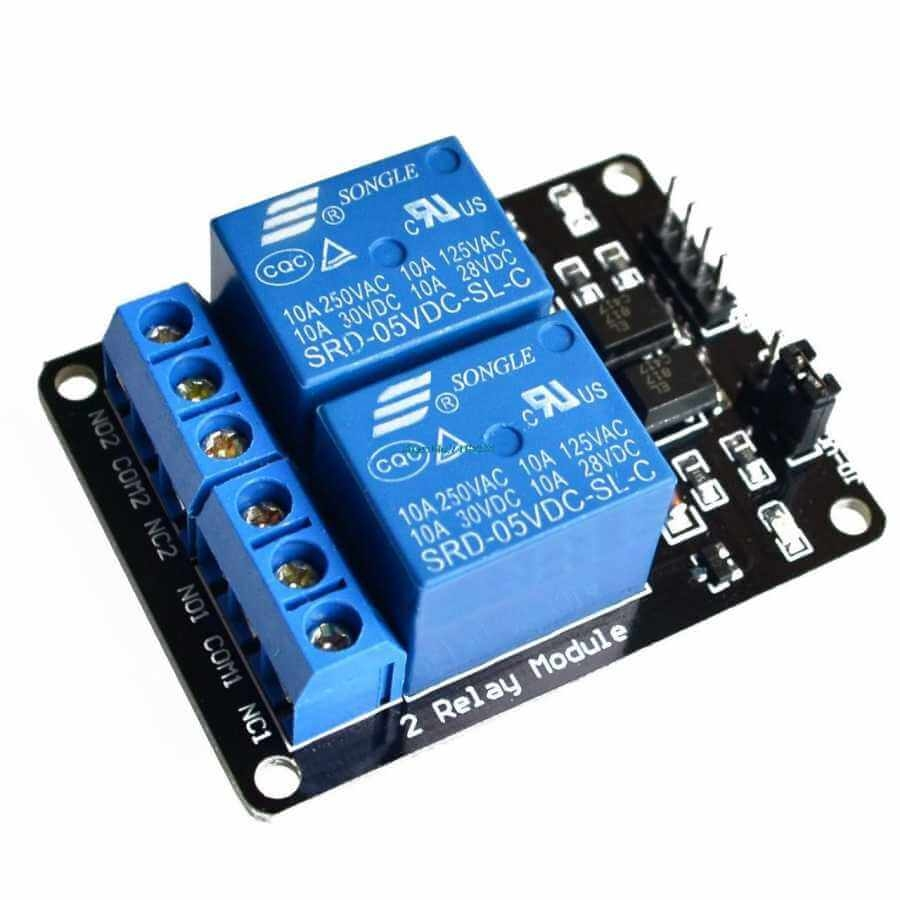
\includegraphics[width=\linewidth]{relay}
		\caption{Placă cu două relee pentru comutarea tensiunii prizei}
		\label{fig:relay}
	\end{subfigure}
	\hfill
	\begin{subfigure}{0.45\textwidth}
		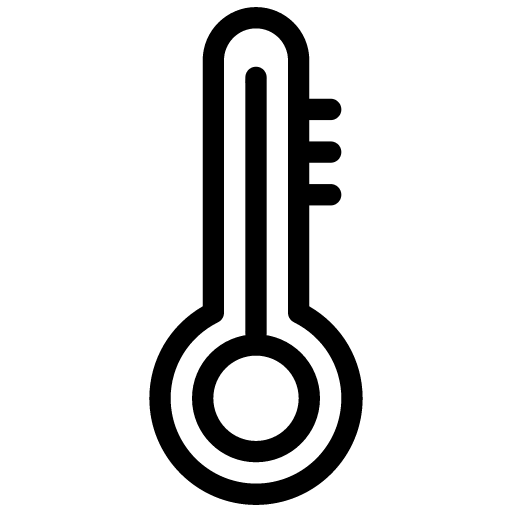
\includegraphics[width=\linewidth]{temperature}
		\caption{Senzor de temperatură și umiditate}
		\label{fig:temperature}
	\end{subfigure}
	\begin{subfigure}{0.45\textwidth}
		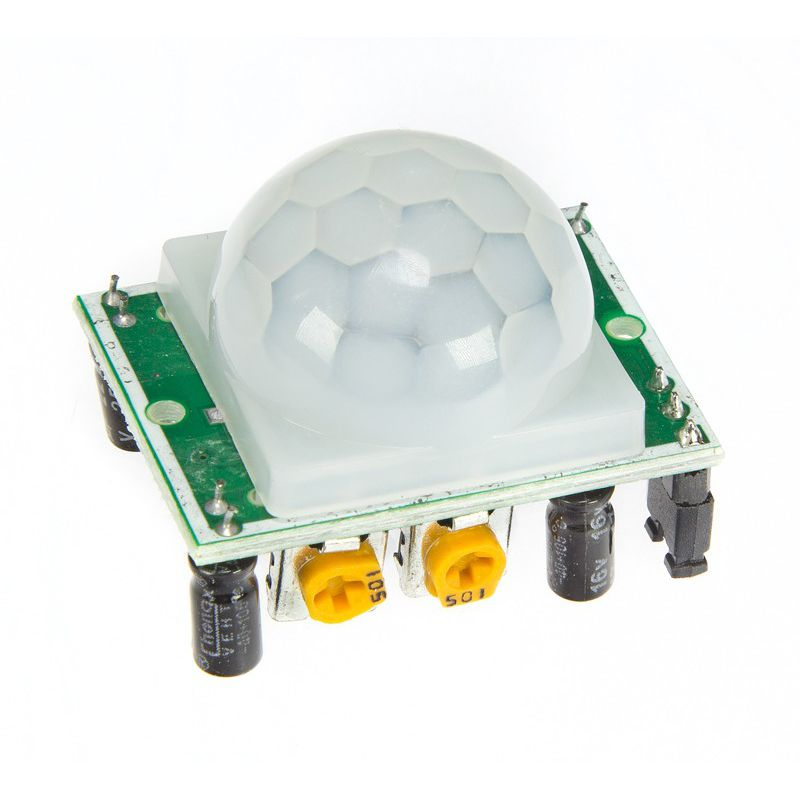
\includegraphics[width=\linewidth]{motion}
		\caption{Senzor de detectarea mișcării}
		\label{fig:motion}
	\end{subfigure}
	\hfill
		\begin{subfigure}{0.45\textwidth}
		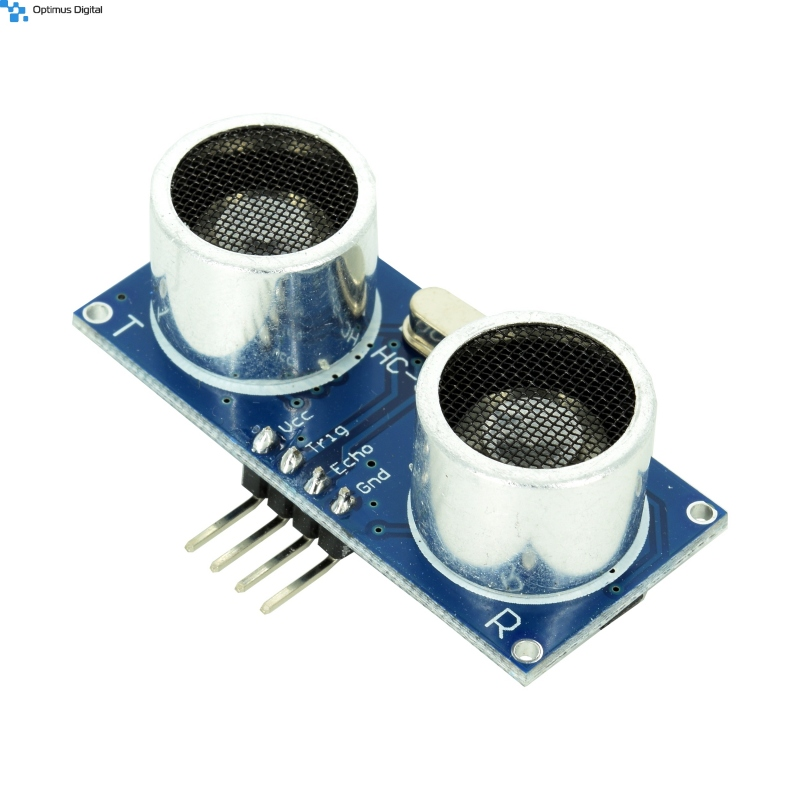
\includegraphics[width=\linewidth]{distance}
		\caption{Senzor de măsurare a distanței}
		\label{fig:distance}
	\end{subfigure}
	\hfill
	\caption{Senzorii folosiți în acest proiect}
	\label{fig:all}
\end{figure}

\section{Concluzii}

Domeniul Smart Home este foarte vast și oferă o gamă largă de oportunități creative. Tehnologia a evoluat rapid, permițând controlul și automatizarea diverselor aspecte ale locuinței, de la iluminat și securitate la gestionarea energiei și confortul locatarilor. 

Moduluele și plăcile folosite se pliază destul de bine pentru aplicările descrise în viitorul capitol, dar întotdeauna acestea vor fi actualizate cu noi funcționalități. Prin urmare, în domeniul caselor inteligente, nu există limite, iar utilizatorii sunt încurajați să-și folosească imaginația și să exploreze noi soluții ce se pliază vieții personale.